\documentclass[11pt]{article}
\usepackage[letterpaper,margin=0.9in]{geometry}
\usepackage{amsmath,amssymb,graphicx}
\usepackage[T1]{fontenc}
\usepackage{mathptmx}
\usepackage{booktabs,longtable,float}
\usepackage{caption}
\usepackage{needspace}
\captionsetup{font=small,labelfont=bf}
\graphicspath{{../figures/}}
\renewcommand{\thetable}{S\arabic{table}}
\renewcommand{\thefigure}{S\arabic{figure}}
\renewcommand{\thesection}{S\arabic{section}}
\newcommand{\Atwo}{\ensuremath{A_2^0\langle r^2\rangle}}
\newcommand{\ndfeb}{\mathrm{Nd_2Fe_{14}B}}
\emergencystretch=2em
\begin{document}
\begin{center}
{\Large\bfseries Supplementary Material}\\[6pt]
{\large Grain-Boundary Environments Reorient the Local $4f$ Susceptibility Axis and Split Light from Heavy Lanthanides in $\ndfeb$}\\[6pt]
Avik Mahata and M. Zakotnik
\end{center}

\section{Structures and embedding definitions}
Tables~\ref{tab:S1} and \ref{tab:S2} give every atom and the lattice vectors of the relaxed 68-atom bulk and 136-atom interface cells. The accompanying \texttt{bulk\_CONTCAR} and \texttt{GB\_CONTCAR} contain the same structures. Table~\ref{tab:S3} lists the rare-earth coordination. The upper half of the interface cell obeys $(x,y,z)\mapsto(-y,x,z+1/2)$ modulo lattice translations, without an additional in-plane translation. The $90^\circ$ rotation is symmetry equivalent at the tetragonal orientation level. The model is a coherent rotational-registry interface, not a representative general high-angle boundary.

The finite-cell calculations in the main figures use bulk atom~2 ($4g$) and interface atom~13 (class A, $4f$ parent). The remaining atoms of one cell carry rare-earth $+3$, Fe 0, and B $-3$ charges. There are 67 and 135 entries, with charge sums $+9e$ and $+21e$, respectively. The quantum ion has charge $+3e$; it is not a point-charge entry. A point-charge sum is therefore a property of the embedding, and is not by itself a validation or invalidation of its local potential. The finite-cell prescription does not reproduce a charge-neutral periodic Madelung potential by construction.

The extended-sphere sensitivity model uses periodic images of the same structures within 18 or 25~\AA{} of the ion, with rare-earth $+3$, Fe $-3/14$, and B $-3$. The residual embedding charge is spread equally over the charges in the outermost 2~\AA{} shell. For example, the 25~\AA{} arrays for Nd at bulk atom~2 and interface atom~13 contain 4768 and 4760 entries; the printed arrays are neutral to their rounding precision. This model changes the Fe charge assignment as well as the truncation geometry and size. Only the comparison of 18 and 25~\AA{} within this prescription is a radius-sensitivity test. An alternative neutral partition uses Fe $-5/14$ and B $-1$. The matched pairs are A (atom~13) versus bulk $4f$ (atom~5), and B (atom~9) versus bulk $4g$ (atom~2). Finite-cell and sphere-model results are labeled separately throughout.

\section{Orbital and magnetic descriptors}
The active spaces, state-average roots and weights, relativistic basis and SOC treatment are specified in the main Methods. The finite-cell calculations use SA-CASSCF; the separate SC-NEVPT2 results are labeled in Table~\ref{tab:S6}. The one-electron AILFT energies $\epsilon_i$ yield the total orbital spread and the orbital gaps $\delta_{\mathrm{orb}}=\epsilon_2-\epsilon_1$ and $\Delta_{\mathrm{orb}}=\epsilon_3-\epsilon_2$. Magnetic excitations instead come from the many-electron QDPT-SOC eigenvalues (Table~\ref{tab:S4}). For Pr and Tb, the table distinguishes the splitting within the lowest pair from the next level; a quasi-doublet need not be a protected degeneracy. The half-filled Gd ground multiplet is weakly split, despite a substantial one-electron orbital spread.

The AILFT matrix is decomposed exactly as $V=\sum_{kq}B^k_qC^k_q$ for $k=2,4,6$, using the angular-momentum matrices printed by ORCA to fix the real-$f$ basis convention. The coefficients satisfy $B^k_{-q}=(-1)^q\overline{B^k_q}$. We report $S_k=[\sum_q|B^k_q|^2/(2k+1)]^{1/2}$ and $\Atwo=B^2_0/2$ in the cell frame with $z\parallel c$. Table~\ref{tab:S5} supplies the finite-cell invariants and axial coefficient; \texttt{wybourne\_Bkq\_all\_runs.csv} supplies the complete complex coefficient sets for the archived calculations, including the additional embedding tests. This CSV is a separate supplementary data file, not an embedded table in the PDF. Figure~\ref{fig:S2} compares rank changes for the finite-cell and matched sphere-model comparisons. Rank decomposition is not a ligand-shell decomposition or a radial-density measurement.

The susceptibility figure uses the tensor-trace response at zero static field, orientationally averaged as $\overline{\chi}_M T=T\,\mathrm{Tr}(\boldsymbol{\chi}_M)/3$. Molar normalization is per rare-earth ion. The main Fig.~3 directions are the eigenvectors of the largest eigenvalues of the directly computed zero-field tensors at 2~K. The Gd susceptibility-axis rotation is $87.08^\circ$ and is included in main Fig.~3; this is not an assignment of first-order orbital anisotropy. The susceptibility axes are evaluated directly from the saved output tensors. Only records with the explicit \texttt{\_bulk} and \texttt{\_GB} labels define the pair; auxiliary \texttt{\_casscf} records are excluded. The archived direction table is based on the principal direction of the printed \texttt{g(OZ/SOC)} contribution, not the full ground-doublet $g$ tensor. With the correct records, that direction indicator gives $87.01^\circ$, $87.34^\circ$, $87.67^\circ$, $87.26^\circ$, and $87.42^\circ$ for Ce, Pr, Nd, Tb, and Dy. The direct 2~K susceptibility directions used in main Fig.~3 differ by less than $0.04^\circ$ from these indicators; the two definitions are not equated. The susceptibility tensor defines the actual linear magnetic response at the stated temperature for both Kramers and non-Kramers ions, whereas the archived indicator uses only one contribution to an effective $g$ matrix. Figure~4 uses the trace of each printed zero-field $\chi_M T$ tensor, from the archived outputs; the separate scalar \texttt{d2E/dB2} column is not substituted for that trace. The orbital maps in main Fig.~5 use the archived orbital-27 cubes for bulk and interface Ce, Pr and Dy. The panel titles give the ion, environment (Bulk or GB), and MO27 file index; the axes have labeled 0.5~\AA{} intervals and 0.25~\AA{} minor ticks. The projected density is $P(a,b)=\int |\psi(a,b,c)|^2\,dc/N$, where $N=\int|\psi|^2d^3r$ is the numerical full-cube norm. All six panels use the common range $0\leq P\leq P_{\max}$, with $P_{\max}=7$~\AA$^{-2}$ and the square-root color coordinate $u=(P/P_{\max})^{1/2}$. The colorbar is labeled in physical $P$ values (\AA$^{-2}$), not in $u$. The same monotonic mapping is applied to every panel to make weak lobes visible; there is no independent panel normalization, density clipping, or change to the integrals and radii. This is a display transformation, not a replacement of the density by an orbital amplitude. Thin black contours outline the projected-density lobes at 0.25, 0.75, and 2.0~\AA$^{-2}$ in every panel. They are isodensity contours, not coordination boundaries. Bicubic interpolation is used only to display the contours; the cube integrals and radii use the original three-dimensional grid. The extent is $r_{\mathrm{rms}}=[\int r^2|\psi|^2d^3r/N]^{1/2}$, measured from the ion using all three-dimensional voxels. The uncorrected grid norms differ from one by less than 0.9\% (Table~\ref{tab:S10}); each density is normalized with its own $N$ before comparison. Projecting the full density avoids an arbitrary slice through an orbital nodal plane. The selected individual eigenorbital is not the many-electron ground-state density, and its angular form can change under mixing of nearly degenerate orbitals. Its extent does not by itself establish a causal radial mechanism for the crystal-field crossover.

\section{Embedding and site sensitivity}
Figure~\ref{fig:S1} and Tables~\ref{tab:S6} and \ref{tab:S7} distinguish finite-cell versus sphere-model changes, the radius test within the sphere model, and matched-site comparisons. The selected-site finite-cell sign crossover is not retained in the matched 25~\AA{} sphere calculations. The sphere model yields a class A increase of the axial term and a smaller class B response, but this does not demonstrate that this charge assignment is uniquely correct. At the tested Nd and Dy sites, changing sphere radius modifies axial parameters by about 5--8\%; changing Fe/B charge partition can modify them by 33--78\%. The 13--14\% change of the ratio of interface atom~13 to bulk atom~2 is not an uncertainty bound on the different matched-sublattice ratios.

The cECP tests in Table~\ref{tab:S8} compare core-repulsion potentials with bare charges at the same def2-TZVP/central-ion-ECP level, using spin-free SA-CASSCF. Every Fe and rare-earth neighbor within 4.0~\AA{} carries its formal charge and, in the capped arm, an embedding ECP but no basis functions. The capped and bare-charge arms differ only by these potentials. Their small differences do not test explicit Fe--$4f$ hybridization, conduction-electron screening, or alternative interface structures. They also do not validate the separate finite-cell charge convention.

\section{Active-space checks and magnetic directions}
The Ce $4f$-parent sphere calculations did not retain seven $f$ active orbitals: one active orbital acquired $6s$ character. A CASCI on free-ion orbitals did not agree adequately with SA-CASSCF where both were available, so the missing Ce class A entries are omitted. This is an active-space limitation, not a calculation of Ce valence in the solid.

For the sphere-model Kramers ions Ce, Nd and Dy, the direction in Table~\ref{tab:S7} is taken directly from the ground-doublet matrix elements of $\mathbf L+g_e\mathbf S$. Directions for the non-Kramers ions Pr and Tb are not assigned in that table because direct temperature-dependent susceptibility tensors were not saved for these sphere calculations. No Gd orbital easy axis is assigned. The main finite-cell directions instead use the saved direct susceptibility tensors for all six ions, with Gd reported as a susceptibility response direction. No fitted ligand-field CI reconstruction is used for the main susceptibility curves, magnetic directions, or orbital-density figure.

\section{Conditional switching-field estimate}
For a single uniaxial coherent-rotation region, $E=K\sin^2\phi-\mu_0M_s H\cos(\phi-\theta)$ yields the Stoner--Wohlfarth loss-of-metastability field $H_{\mathrm{sw}}/H_A=(|\cos\theta|^{2/3}+|\sin\theta|^{2/3})^{-3/2}$, with $H_A=2K/(\mu_0 M_s)$. Table~\ref{tab:S9} evaluates this dimensionless expression for the finite-cell susceptibility-axis angles, assuming the applied field is along the bulk response axis. The result is not the hysteretic coercivity along a hard direction, and it is not a spatially resolved nucleation calculation. It omits exchange between the region and host, demagnetizing fields, changes of $K$ or $M_s$, and nonuniform reversal. No value of $K$ is inferred from the orbital-energy spread, and no absolute coercive field is assigned.

\begin{figure}[H]
\centering
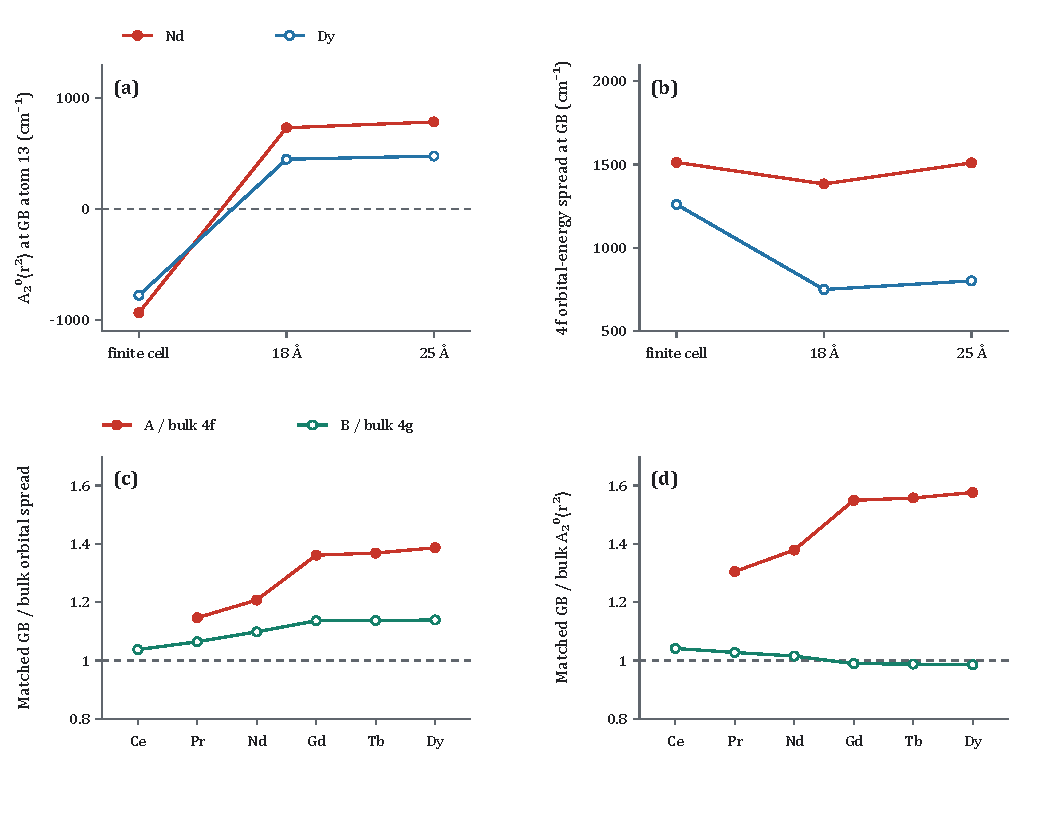
\includegraphics[width=\linewidth]{Figure_S1.pdf}
\caption{Embedding and site comparisons. (a) Axial parameter at interface atom~13 and (b) one-electron orbital-energy spread for Nd and Dy in the finite-cell model and the 18 and 25~\AA{} sphere models. The first step changes charge assignment as well as truncation; the second step tests radius within one charge convention. (c) Orbital-spread ratios and (d) axial-parameter ratios for matched pairs in the 25~\AA{} sphere model. The Ce class A pair is absent because the active-space optimization was unstable. Lines guide the eye.}\label{fig:S1}
\end{figure}

\begin{figure}[H]
\centering
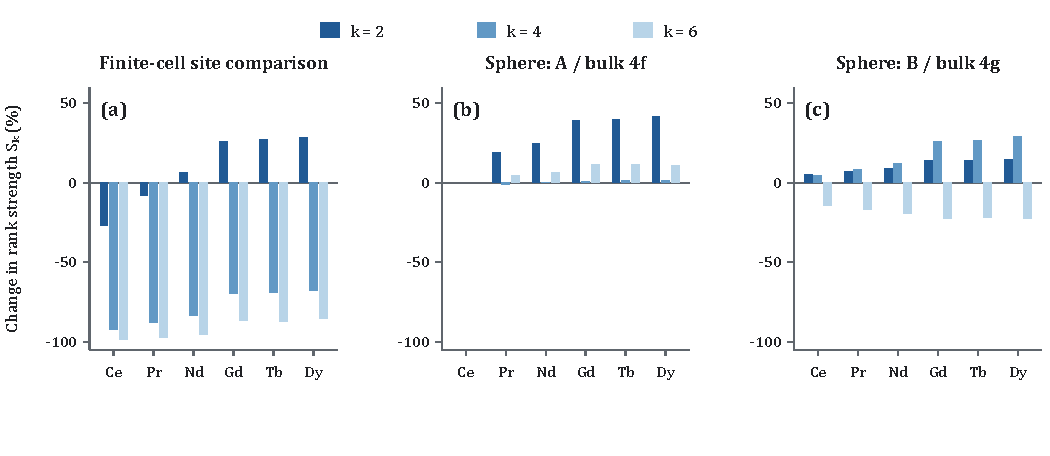
\includegraphics[width=\linewidth]{Figure_S2.pdf}
\caption{Relative changes of exact rank invariants $S_k$ ($k=2,4,6$). (a) Finite-cell selected-site comparison, bulk atom~2 versus interface atom~13; (b) matched class A versus bulk $4f$ and (c) matched class B versus bulk $4g$ in the 25~\AA{} sphere model. The different patterns show that the finite-cell sign crossover cannot be treated as an embedding-independent geometric effect. The decomposition does not isolate radial contraction.}\label{fig:S2}
\end{figure}

\clearpage
\begin{longtable}{rlrrrrrrl}
\caption{Relaxed bulk Nd$_8$Fe$_{56}$B$_4$ supercell (68 atoms, space group $P4_2/mnm$). Lattice vectors (\AA): $a_1$ = (8.756856, 0.000000, 0.000000), $a_2$ = (-0.000000, 8.756856, 0.000000), $a_3$ = (-0.000000, -0.000000, 12.129949). Fractional ($x,y,z$) and Cartesian ($X,Y,Z$, \AA) coordinates; atom indices are those used in the main text.}\label{tab:S1}\\
\toprule
\# & El. & $x$ & $y$ & $z$ & $X$ & $Y$ & $Z$ & Site \\
\midrule
\endfirsthead
\toprule
\# & El. & $x$ & $y$ & $z$ & $X$ & $Y$ & $Z$ & Site \\
\midrule
\endhead
1 & Nd & 0.85705 & 0.14295 & -0.00000 & 7.5051 & 1.2518 & 0.0000 & 4g \\
2 & Nd & 0.35705 & 0.35705 & 0.50000 & 3.1267 & 3.1267 & 6.0650 & 4g \\
3 & Nd & 0.64295 & 0.64295 & 0.50000 & 5.6302 & 5.6302 & 6.0650 & 4g \\
4 & Nd & 0.14295 & 0.85705 & -0.00000 & 1.2518 & 7.5051 & 0.0000 & 4g \\
5 & Nd & 0.73144 & 0.73144 & -0.00000 & 6.4051 & 6.4051 & 0.0000 & 4f \\
6 & Nd & 0.76856 & 0.23144 & 0.50000 & 6.7302 & 2.0267 & 6.0650 & 4f \\
7 & Nd & 0.23144 & 0.76856 & 0.50000 & 2.0267 & 6.7302 & 6.0650 & 4f \\
8 & Nd & 0.26856 & 0.26856 & -0.00000 & 2.3517 & 2.3517 & 0.0000 & 4f \\
9 & Fe & 0.56740 & 0.22461 & 0.12756 & 4.9687 & 1.9669 & 1.5473 &  \\
10 & Fe & 0.43260 & 0.77539 & 0.12756 & 3.7882 & 6.7899 & 1.5473 &  \\
11 & Fe & 0.22461 & 0.56740 & 0.87244 & 1.9669 & 4.9687 & 10.5826 &  \\
12 & Fe & 0.72461 & 0.93260 & 0.62756 & 6.3453 & 8.1666 & 7.6123 &  \\
13 & Fe & 0.27539 & 0.06740 & 0.62756 & 2.4115 & 0.5902 & 7.6123 &  \\
14 & Fe & 0.93260 & 0.72461 & 0.37244 & 8.1666 & 6.3453 & 4.5176 &  \\
15 & Fe & 0.06740 & 0.27539 & 0.37244 & 0.5902 & 2.4115 & 4.5176 &  \\
16 & Fe & 0.77539 & 0.43260 & 0.87244 & 6.7899 & 3.7882 & 10.5826 &  \\
17 & Fe & 0.43260 & 0.77539 & 0.87244 & 3.7882 & 6.7899 & 10.5826 &  \\
18 & Fe & 0.56740 & 0.22461 & 0.87244 & 4.9687 & 1.9669 & 10.5826 &  \\
19 & Fe & 0.77539 & 0.43260 & 0.12756 & 6.7899 & 3.7882 & 1.5473 &  \\
20 & Fe & 0.27539 & 0.06740 & 0.37244 & 2.4115 & 0.5902 & 4.5176 &  \\
21 & Fe & 0.72461 & 0.93260 & 0.37244 & 6.3453 & 8.1666 & 4.5176 &  \\
22 & Fe & 0.06740 & 0.27539 & 0.62756 & 0.5902 & 2.4115 & 7.6123 &  \\
23 & Fe & 0.93260 & 0.72461 & 0.62756 & 8.1666 & 6.3453 & 7.6123 &  \\
24 & Fe & 0.22461 & 0.56740 & 0.12756 & 1.9669 & 4.9687 & 1.5473 &  \\
25 & Fe & 0.35996 & 0.03683 & 0.17626 & 3.1521 & 0.3225 & 2.1381 &  \\
26 & Fe & 0.64004 & 0.96317 & 0.17626 & 5.6047 & 8.4343 & 2.1381 &  \\
27 & Fe & 0.03683 & 0.35996 & 0.82374 & 0.3225 & 3.1521 & 9.9919 &  \\
28 & Fe & 0.53683 & 0.14004 & 0.67626 & 4.7010 & 1.2263 & 8.2031 &  \\
29 & Fe & 0.46317 & 0.85996 & 0.67626 & 4.0559 & 7.5306 & 8.2031 &  \\
30 & Fe & 0.14004 & 0.53683 & 0.32374 & 1.2263 & 4.7010 & 3.9269 &  \\
31 & Fe & 0.85996 & 0.46317 & 0.32374 & 7.5306 & 4.0559 & 3.9269 &  \\
32 & Fe & 0.96317 & 0.64004 & 0.82374 & 8.4343 & 5.6047 & 9.9919 &  \\
33 & Fe & 0.64004 & 0.96317 & 0.82374 & 5.6047 & 8.4343 & 9.9919 &  \\
34 & Fe & 0.35996 & 0.03683 & 0.82374 & 3.1521 & 0.3225 & 9.9919 &  \\
35 & Fe & 0.96317 & 0.64004 & 0.17626 & 8.4343 & 5.6047 & 2.1381 &  \\
36 & Fe & 0.46317 & 0.85996 & 0.32374 & 4.0559 & 7.5306 & 3.9269 &  \\
37 & Fe & 0.53683 & 0.14004 & 0.32374 & 4.7010 & 1.2263 & 3.9269 &  \\
38 & Fe & 0.85996 & 0.46317 & 0.67626 & 7.5306 & 4.0559 & 8.2031 &  \\
39 & Fe & 0.14004 & 0.53683 & 0.67626 & 1.2263 & 4.7010 & 8.2031 &  \\
40 & Fe & 0.03683 & 0.35996 & 0.17626 & 0.3225 & 3.1521 & 2.1381 &  \\
41 & Fe & 0.90221 & 0.90221 & 0.79526 & 7.9006 & 7.9006 & 9.6465 &  \\
42 & Fe & 0.09779 & 0.09779 & 0.79526 & 0.8563 & 0.8563 & 9.6465 &  \\
43 & Fe & 0.90221 & 0.90221 & 0.20474 & 7.9006 & 7.9006 & 2.4835 &  \\
44 & Fe & 0.40221 & 0.59779 & 0.29526 & 3.5221 & 5.2347 & 3.5815 &  \\
45 & Fe & 0.59779 & 0.40221 & 0.29526 & 5.2347 & 3.5221 & 3.5815 &  \\
46 & Fe & 0.59779 & 0.40221 & 0.70474 & 5.2347 & 3.5221 & 8.5485 &  \\
47 & Fe & 0.40221 & 0.59779 & 0.70474 & 3.5221 & 5.2347 & 8.5485 &  \\
48 & Fe & 0.09779 & 0.09779 & 0.20474 & 0.8563 & 0.8563 & 2.4835 &  \\
49 & Fe & 0.68217 & 0.68217 & 0.75430 & 5.9737 & 5.9737 & 9.1496 &  \\
50 & Fe & 0.31783 & 0.31783 & 0.75430 & 2.7832 & 2.7832 & 9.1496 &  \\
51 & Fe & 0.68217 & 0.68217 & 0.24570 & 5.9737 & 5.9737 & 2.9804 &  \\
52 & Fe & 0.18217 & 0.81783 & 0.25430 & 1.5952 & 7.1616 & 3.0846 &  \\
53 & Fe & 0.81783 & 0.18217 & 0.25430 & 7.1616 & 1.5952 & 3.0846 &  \\
54 & Fe & 0.81783 & 0.18217 & 0.74570 & 7.1616 & 1.5952 & 9.0453 &  \\
55 & Fe & 0.18217 & 0.81783 & 0.74570 & 1.5952 & 7.1616 & 9.0453 &  \\
56 & Fe & 0.31783 & 0.31783 & 0.24570 & 2.7832 & 2.7832 & 2.9804 &  \\
57 & Fe & -0.00000 & 0.00000 & 0.61492 & 0.0000 & 0.0000 & 7.4589 &  \\
58 & Fe & 0.50000 & 0.50000 & 0.11492 & 4.3784 & 4.3784 & 1.3939 &  \\
59 & Fe & 0.50000 & 0.50000 & 0.88508 & 4.3784 & 4.3784 & 10.7360 &  \\
60 & Fe & -0.00000 & 0.00000 & 0.38508 & 0.0000 & 0.0000 & 4.6710 &  \\
61 & Fe & 0.50000 & 0.00000 & -0.00000 & 4.3784 & 0.0000 & 0.0000 &  \\
62 & Fe & 0.50000 & 0.00000 & 0.50000 & 4.3784 & 0.0000 & 6.0650 &  \\
63 & Fe & -0.00000 & 0.50000 & 0.50000 & -0.0000 & 4.3784 & 6.0650 &  \\
64 & Fe & -0.00000 & 0.50000 & -0.00000 & -0.0000 & 4.3784 & 0.0000 &  \\
65 & B & 0.62335 & 0.37665 & -0.00000 & 5.4586 & 3.2982 & 0.0000 &  \\
66 & B & 0.12335 & 0.12335 & 0.50000 & 1.0802 & 1.0802 & 6.0650 &  \\
67 & B & 0.87665 & 0.87665 & 0.50000 & 7.6767 & 7.6767 & 6.0650 &  \\
68 & B & 0.37665 & 0.62335 & -0.00000 & 3.2982 & 5.4586 & 0.0000 &  \\
\bottomrule
\end{longtable}

\begin{longtable}{rlrrrrrrl}
\caption{Relaxed $90^\circ$ [001] twist grain-boundary supercell Nd$_{16}$Fe$_{112}$B$_8$ (136 atoms). Interface planes at $z = 0$ and $z = 1/2$; the rotation specifies the coherent registry construction (Section~S1). Lattice vectors (\AA): $a_1$ = (8.776004, 0.000000, 0.000000), $a_2$ = (-0.000000, 8.776004, 0.000000), $a_3$ = (0.000000, 0.000000, 24.238864). Fractional ($x,y,z$) and Cartesian ($X,Y,Z$, \AA) coordinates; atom indices are those used in the main text.}\label{tab:S2}\\
\toprule
\# & El. & $x$ & $y$ & $z$ & $X$ & $Y$ & $Z$ & Site \\
\midrule
\endfirsthead
\toprule
\# & El. & $x$ & $y$ & $z$ & $X$ & $Y$ & $Z$ & Site \\
\midrule
\endhead
1 & Nd & 0.84544 & 0.15456 & 0.00216 & 7.4196 & 1.3564 & 0.0523 & class B \\
2 & Nd & 0.35610 & 0.35610 & 0.25023 & 3.1251 & 3.1251 & 6.0653 & class C \\
3 & Nd & 0.64390 & 0.64390 & 0.25023 & 5.6509 & 5.6509 & 6.0653 & class C \\
4 & Nd & 0.15456 & 0.84544 & 0.00216 & 1.3564 & 7.4196 & 0.0523 & class B \\
5 & Nd & 0.75274 & 0.75274 & -0.00146 & 6.6061 & 6.6061 & -0.0355 & class A \\
6 & Nd & 0.76445 & 0.23555 & 0.25005 & 6.7088 & 2.0672 & 6.0609 & class D \\
7 & Nd & 0.23555 & 0.76445 & 0.25005 & 2.0672 & 6.7088 & 6.0609 & class D \\
8 & Nd & 0.24726 & 0.24726 & -0.00146 & 2.1699 & 2.1699 & -0.0355 & class A \\
9 & Nd & 0.84544 & 0.84544 & 0.50216 & 7.4196 & 7.4196 & 12.1717 & class B \\
10 & Nd & 0.64390 & 0.35610 & 0.75023 & 5.6509 & 3.1251 & 18.1847 & class C \\
11 & Nd & 0.35610 & 0.64390 & 0.75023 & 3.1251 & 5.6509 & 18.1847 & class C \\
12 & Nd & 0.15456 & 0.15456 & 0.50216 & 1.3564 & 1.3564 & 12.1717 & class B \\
13 & Nd & 0.24726 & 0.75274 & 0.49854 & 2.1699 & 6.6061 & 12.0839 & class A \\
14 & Nd & 0.76445 & 0.76445 & 0.75005 & 6.7088 & 6.7088 & 18.1803 & class D \\
15 & Nd & 0.23555 & 0.23555 & 0.75005 & 2.0672 & 2.0672 & 18.1803 & class D \\
16 & Nd & 0.75274 & 0.24726 & 0.49854 & 6.6061 & 2.1699 & 12.0839 & class A \\
17 & Fe & 0.55952 & 0.22634 & 0.06334 & 4.9104 & 1.9864 & 1.5353 &  \\
18 & Fe & 0.44048 & 0.77366 & 0.06334 & 3.8656 & 6.7897 & 1.5353 &  \\
19 & Fe & 0.22916 & 0.47739 & 0.44344 & 2.0111 & 4.1895 & 10.7484 &  \\
20 & Fe & 0.72310 & 0.93917 & 0.31070 & 6.3459 & 8.2422 & 7.5310 &  \\
21 & Fe & 0.27690 & 0.06083 & 0.31070 & 2.4301 & 0.5338 & 7.5310 &  \\
22 & Fe & 0.93460 & 0.72426 & 0.18595 & 8.2021 & 6.3562 & 4.5071 &  \\
23 & Fe & 0.06540 & 0.27574 & 0.18595 & 0.5739 & 2.4199 & 4.5071 &  \\
24 & Fe & 0.77084 & 0.52261 & 0.44344 & 6.7649 & 4.5865 & 10.7484 &  \\
25 & Fe & 0.52261 & 0.77084 & 0.44344 & 4.5865 & 6.7649 & 10.7484 &  \\
26 & Fe & 0.47739 & 0.22916 & 0.44344 & 4.1895 & 2.0111 & 10.7484 &  \\
27 & Fe & 0.77366 & 0.44048 & 0.06334 & 6.7897 & 3.8656 & 1.5353 &  \\
28 & Fe & 0.27574 & 0.06540 & 0.18595 & 2.4199 & 0.5739 & 4.5071 &  \\
29 & Fe & 0.72426 & 0.93460 & 0.18595 & 6.3562 & 8.2021 & 4.5071 &  \\
30 & Fe & 0.06083 & 0.27690 & 0.31070 & 0.5338 & 2.4301 & 7.5310 &  \\
31 & Fe & 0.93917 & 0.72310 & 0.31070 & 8.2422 & 6.3459 & 7.5310 &  \\
32 & Fe & 0.22634 & 0.55952 & 0.06334 & 1.9864 & 4.9104 & 1.5353 &  \\
33 & Fe & 0.35905 & 0.03426 & 0.08832 & 3.1510 & 0.3007 & 2.1407 &  \\
34 & Fe & 0.64095 & 0.96574 & 0.08832 & 5.6250 & 8.4753 & 2.1407 &  \\
35 & Fe & 0.01341 & 0.35651 & 0.41034 & 0.1177 & 3.1287 & 9.9463 &  \\
36 & Fe & 0.53025 & 0.14444 & 0.33880 & 4.6535 & 1.2676 & 8.2121 &  \\
37 & Fe & 0.46975 & 0.85556 & 0.33880 & 4.1225 & 7.5084 & 8.2121 &  \\
38 & Fe & 0.14078 & 0.53525 & 0.16169 & 1.2355 & 4.6974 & 3.9192 &  \\
39 & Fe & 0.85922 & 0.46475 & 0.16169 & 7.5405 & 4.0786 & 3.9192 &  \\
40 & Fe & 0.98659 & 0.64349 & 0.41034 & 8.6583 & 5.6473 & 9.9463 &  \\
41 & Fe & 0.64349 & 0.98659 & 0.41034 & 5.6473 & 8.6583 & 9.9463 &  \\
42 & Fe & 0.35651 & 0.01341 & 0.41034 & 3.1287 & 0.1177 & 9.9463 &  \\
43 & Fe & 0.96574 & 0.64095 & 0.08832 & 8.4753 & 5.6250 & 2.1407 &  \\
44 & Fe & 0.46475 & 0.85922 & 0.16169 & 4.0786 & 7.5405 & 3.9192 &  \\
45 & Fe & 0.53525 & 0.14078 & 0.16169 & 4.6974 & 1.2355 & 3.9192 &  \\
46 & Fe & 0.85556 & 0.46975 & 0.33880 & 7.5084 & 4.1225 & 8.2121 &  \\
47 & Fe & 0.14444 & 0.53025 & 0.33880 & 1.2676 & 4.6535 & 8.2121 &  \\
48 & Fe & 0.03426 & 0.35905 & 0.08832 & 0.3007 & 3.1510 & 2.1407 &  \\
49 & Fe & 0.90461 & 0.90461 & 0.38996 & 7.9388 & 7.9388 & 9.4522 &  \\
50 & Fe & 0.09539 & 0.09539 & 0.38996 & 0.8372 & 0.8372 & 9.4522 &  \\
51 & Fe & 0.90319 & 0.90319 & 0.10257 & 7.9264 & 7.9264 & 2.4862 &  \\
52 & Fe & 0.40268 & 0.59732 & 0.14701 & 3.5339 & 5.2421 & 3.5633 &  \\
53 & Fe & 0.59732 & 0.40268 & 0.14701 & 5.2421 & 3.5339 & 3.5633 &  \\
54 & Fe & 0.59813 & 0.40187 & 0.36057 & 5.2492 & 3.5268 & 8.7397 &  \\
55 & Fe & 0.40187 & 0.59813 & 0.36057 & 3.5268 & 5.2492 & 8.7397 &  \\
56 & Fe & 0.09681 & 0.09681 & 0.10257 & 0.8496 & 0.8496 & 2.4862 &  \\
57 & Fe & 0.70322 & 0.70322 & 0.37353 & 6.1715 & 6.1715 & 9.0539 &  \\
58 & Fe & 0.29678 & 0.29678 & 0.37353 & 2.6045 & 2.6045 & 9.0539 &  \\
59 & Fe & 0.68486 & 0.68486 & 0.12240 & 6.0103 & 6.0103 & 2.9668 &  \\
60 & Fe & 0.18508 & 0.81492 & 0.12707 & 1.6242 & 7.1518 & 3.0800 &  \\
61 & Fe & 0.81492 & 0.18508 & 0.12707 & 7.1518 & 1.6242 & 3.0800 &  \\
62 & Fe & 0.81310 & 0.18690 & 0.37166 & 7.1358 & 1.6402 & 9.0087 &  \\
63 & Fe & 0.18690 & 0.81310 & 0.37166 & 1.6402 & 7.1358 & 9.0087 &  \\
64 & Fe & 0.31514 & 0.31514 & 0.12240 & 2.7657 & 2.7657 & 2.9668 &  \\
65 & Fe & -0.00000 & -0.00000 & 0.30390 & 0.0000 & 0.0000 & 7.3663 &  \\
66 & Fe & 0.50000 & 0.50000 & 0.05696 & 4.3880 & 4.3880 & 1.3805 &  \\
67 & Fe & 0.50000 & 0.50000 & 0.44588 & 4.3880 & 4.3880 & 10.8077 &  \\
68 & Fe & -0.00000 & -0.00000 & 0.19182 & 0.0000 & 0.0000 & 4.6496 &  \\
69 & Fe & 0.50000 & -0.00000 & 0.00097 & 4.3880 & 0.0000 & 0.0236 &  \\
70 & Fe & 0.50000 & -0.00000 & 0.24982 & 4.3880 & 0.0000 & 6.0554 &  \\
71 & Fe & -0.00000 & 0.50000 & 0.24982 & -0.0000 & 4.3880 & 6.0554 &  \\
72 & Fe & -0.00000 & 0.50000 & 0.00097 & -0.0000 & 4.3880 & 0.0236 &  \\
73 & Fe & 0.77366 & 0.55952 & 0.56334 & 6.7897 & 4.9104 & 13.6548 &  \\
74 & Fe & 0.22634 & 0.44048 & 0.56334 & 1.9864 & 3.8656 & 13.6548 &  \\
75 & Fe & 0.52261 & 0.22916 & 0.94344 & 4.5865 & 2.0111 & 22.8678 &  \\
76 & Fe & 0.06083 & 0.72310 & 0.81070 & 0.5338 & 6.3459 & 19.6504 &  \\
77 & Fe & 0.93917 & 0.27690 & 0.81070 & 8.2422 & 2.4301 & 19.6504 &  \\
78 & Fe & 0.27574 & 0.93460 & 0.68595 & 2.4199 & 8.2021 & 16.6266 &  \\
79 & Fe & 0.72426 & 0.06540 & 0.68595 & 6.3562 & 0.5739 & 16.6266 &  \\
80 & Fe & 0.47739 & 0.77084 & 0.94344 & 4.1895 & 6.7649 & 22.8678 &  \\
81 & Fe & 0.22916 & 0.52261 & 0.94344 & 2.0111 & 4.5865 & 22.8678 &  \\
82 & Fe & 0.77084 & 0.47739 & 0.94344 & 6.7649 & 4.1895 & 22.8678 &  \\
83 & Fe & 0.55952 & 0.77366 & 0.56334 & 4.9104 & 6.7897 & 13.6548 &  \\
84 & Fe & 0.93460 & 0.27574 & 0.68595 & 8.2021 & 2.4199 & 16.6266 &  \\
85 & Fe & 0.06540 & 0.72426 & 0.68595 & 0.5739 & 6.3562 & 16.6266 &  \\
86 & Fe & 0.72310 & 0.06083 & 0.81070 & 6.3459 & 0.5338 & 19.6504 &  \\
87 & Fe & 0.27690 & 0.93917 & 0.81070 & 2.4301 & 8.2422 & 19.6504 &  \\
88 & Fe & 0.44048 & 0.22634 & 0.56334 & 3.8656 & 1.9864 & 13.6548 &  \\
89 & Fe & 0.96574 & 0.35905 & 0.58832 & 8.4753 & 3.1510 & 14.2602 &  \\
90 & Fe & 0.03426 & 0.64095 & 0.58832 & 0.3007 & 5.6250 & 14.2602 &  \\
91 & Fe & 0.64349 & 0.01341 & 0.91034 & 5.6473 & 0.1177 & 22.0657 &  \\
92 & Fe & 0.85556 & 0.53025 & 0.83880 & 7.5084 & 4.6535 & 20.3316 &  \\
93 & Fe & 0.14444 & 0.46975 & 0.83880 & 1.2676 & 4.1225 & 20.3316 &  \\
94 & Fe & 0.46475 & 0.14078 & 0.66169 & 4.0786 & 1.2355 & 16.0387 &  \\
95 & Fe & 0.53525 & 0.85922 & 0.66169 & 4.6974 & 7.5405 & 16.0387 &  \\
96 & Fe & 0.35651 & 0.98659 & 0.91034 & 3.1287 & 8.6583 & 22.0657 &  \\
97 & Fe & 0.01341 & 0.64349 & 0.91034 & 0.1177 & 5.6473 & 22.0657 &  \\
98 & Fe & 0.98659 & 0.35651 & 0.91034 & 8.6583 & 3.1287 & 22.0657 &  \\
99 & Fe & 0.35905 & 0.96574 & 0.58832 & 3.1510 & 8.4753 & 14.2602 &  \\
100 & Fe & 0.14078 & 0.46475 & 0.66169 & 1.2355 & 4.0786 & 16.0387 &  \\
101 & Fe & 0.85922 & 0.53525 & 0.66169 & 7.5405 & 4.6974 & 16.0387 &  \\
102 & Fe & 0.53025 & 0.85556 & 0.83880 & 4.6535 & 7.5084 & 20.3316 &  \\
103 & Fe & 0.46975 & 0.14444 & 0.83880 & 4.1225 & 1.2676 & 20.3316 &  \\
104 & Fe & 0.64095 & 0.03426 & 0.58832 & 5.6250 & 0.3007 & 14.2602 &  \\
105 & Fe & 0.09539 & 0.90461 & 0.88996 & 0.8372 & 7.9388 & 21.5716 &  \\
106 & Fe & 0.90461 & 0.09539 & 0.88996 & 7.9388 & 0.8372 & 21.5716 &  \\
107 & Fe & 0.09681 & 0.90319 & 0.60257 & 0.8496 & 7.9264 & 14.6057 &  \\
108 & Fe & 0.40268 & 0.40268 & 0.64701 & 3.5339 & 3.5339 & 15.6828 &  \\
109 & Fe & 0.59732 & 0.59732 & 0.64701 & 5.2421 & 5.2421 & 15.6828 &  \\
110 & Fe & 0.59813 & 0.59813 & 0.86057 & 5.2492 & 5.2492 & 20.8592 &  \\
111 & Fe & 0.40187 & 0.40187 & 0.86057 & 3.5268 & 3.5268 & 20.8592 &  \\
112 & Fe & 0.90319 & 0.09681 & 0.60257 & 7.9264 & 0.8496 & 14.6057 &  \\
113 & Fe & 0.29678 & 0.70322 & 0.87353 & 2.6045 & 6.1715 & 21.1733 &  \\
114 & Fe & 0.70322 & 0.29678 & 0.87353 & 6.1715 & 2.6045 & 21.1733 &  \\
115 & Fe & 0.31514 & 0.68486 & 0.62240 & 2.7657 & 6.0103 & 15.0862 &  \\
116 & Fe & 0.18508 & 0.18508 & 0.62707 & 1.6242 & 1.6242 & 15.1994 &  \\
117 & Fe & 0.81492 & 0.81492 & 0.62707 & 7.1518 & 7.1518 & 15.1994 &  \\
118 & Fe & 0.81310 & 0.81310 & 0.87166 & 7.1358 & 7.1358 & 21.1281 &  \\
119 & Fe & 0.18690 & 0.18690 & 0.87166 & 1.6402 & 1.6402 & 21.1281 &  \\
120 & Fe & 0.68486 & 0.31514 & 0.62240 & 6.0103 & 2.7657 & 15.0862 &  \\
121 & Fe & -0.00000 & -0.00000 & 0.80390 & 0.0000 & 0.0000 & 19.4857 &  \\
122 & Fe & 0.50000 & 0.50000 & 0.55696 & 4.3880 & 4.3880 & 13.5000 &  \\
123 & Fe & 0.50000 & 0.50000 & 0.94588 & 4.3880 & 4.3880 & 22.9271 &  \\
124 & Fe & -0.00000 & -0.00000 & 0.69182 & 0.0000 & 0.0000 & 16.7690 &  \\
125 & Fe & -0.00000 & 0.50000 & 0.50097 & -0.0000 & 4.3880 & 12.1430 &  \\
126 & Fe & -0.00000 & 0.50000 & 0.74982 & -0.0000 & 4.3880 & 18.1748 &  \\
127 & Fe & 0.50000 & -0.00000 & 0.74982 & 4.3880 & 0.0000 & 18.1748 &  \\
128 & Fe & 0.50000 & -0.00000 & 0.50097 & 4.3880 & 0.0000 & 12.1430 &  \\
129 & B & 0.62371 & 0.37629 & 0.00056 & 5.4737 & 3.3023 & 0.0135 &  \\
130 & B & 0.12540 & 0.12540 & 0.24847 & 1.1005 & 1.1005 & 6.0226 &  \\
131 & B & 0.87460 & 0.87460 & 0.24847 & 7.6755 & 7.6755 & 6.0226 &  \\
132 & B & 0.37629 & 0.62371 & 0.00056 & 3.3023 & 5.4737 & 0.0135 &  \\
133 & B & 0.62371 & 0.62371 & 0.50056 & 5.4737 & 5.4737 & 12.1330 &  \\
134 & B & 0.87460 & 0.12540 & 0.74847 & 7.6755 & 1.1005 & 18.1420 &  \\
135 & B & 0.12540 & 0.87460 & 0.74847 & 1.1005 & 7.6755 & 18.1420 &  \\
136 & B & 0.37629 & 0.37629 & 0.50056 & 3.3023 & 3.3023 & 12.1330 &  \\
\bottomrule
\end{longtable}

\begin{longtable}{llllcl}
\caption{Coordination of every rare-earth site: number of Fe neighbors within 3.3~\AA{} and the eight shortest RE--Fe distances (periodic images included).}\label{tab:S3}\\
\toprule
Environment & Atom & Site & $z$ (\AA) & $N_{\mathrm{Fe}}$ & shortest RE--Fe distances (\AA) \\
\midrule
\endfirsthead
\toprule
Environment & Atom & Site & $z$ (\AA) & $N_{\mathrm{Fe}}$ & shortest RE--Fe distances (\AA) \\
\midrule
\endhead
bulk & 1 & 4g & 0.000 & 14 & 3.056, 3.056, 3.056, 3.056, 3.123, 3.123, 3.265, 3.265 \\
bulk & 2 & 4g & 6.065 & 14 & 3.056, 3.056, 3.056, 3.056, 3.123, 3.123, 3.265, 3.265 \\
bulk & 3 & 4g & 6.065 & 14 & 3.056, 3.056, 3.056, 3.056, 3.123, 3.123, 3.265, 3.265 \\
bulk & 4 & 4g & 0.000 & 14 & 3.056, 3.056, 3.056, 3.056, 3.123, 3.123, 3.265, 3.265 \\
bulk & 5 & 4f & 0.000 & 16 & 3.042, 3.042, 3.054, 3.054, 3.054, 3.054, 3.064, 3.064 \\
bulk & 6 & 4f & 6.065 & 16 & 3.042, 3.042, 3.054, 3.054, 3.054, 3.054, 3.064, 3.064 \\
bulk & 7 & 4f & 6.065 & 16 & 3.042, 3.042, 3.054, 3.054, 3.054, 3.054, 3.064, 3.064 \\
bulk & 8 & 4f & 0.000 & 16 & 3.042, 3.042, 3.054, 3.054, 3.054, 3.054, 3.064, 3.064 \\
GB & 1 & class B & 0.052 & 10 & 2.817, 2.982, 2.982, 3.051, 3.103, 3.103, 3.214, 3.214 \\
GB & 2 & class C & 6.065 & 10 & 3.057, 3.057, 3.071, 3.071, 3.078, 3.140, 3.224, 3.224 \\
GB & 3 & class C & 6.065 & 10 & 3.057, 3.057, 3.071, 3.071, 3.078, 3.140, 3.224, 3.224 \\
GB & 4 & class B & 0.052 & 10 & 2.817, 2.982, 2.982, 3.051, 3.103, 3.103, 3.214, 3.214 \\
GB & 5 & class A & -0.035 & 13 & 2.766, 2.766, 3.032, 3.032, 3.104, 3.104, 3.118, 3.138 \\
GB & 6 & class D & 6.061 & 15 & 3.009, 3.010, 3.010, 3.046, 3.054, 3.054, 3.081, 3.081 \\
GB & 7 & class D & 6.061 & 15 & 3.009, 3.010, 3.010, 3.046, 3.054, 3.054, 3.081, 3.081 \\
GB & 8 & class A & -0.035 & 13 & 2.766, 2.766, 3.032, 3.032, 3.104, 3.104, 3.118, 3.138 \\
GB & 9 & class B & 12.172 & 10 & 2.817, 2.982, 2.982, 3.051, 3.103, 3.103, 3.214, 3.214 \\
GB & 10 & class C & 18.185 & 10 & 3.057, 3.057, 3.071, 3.071, 3.078, 3.140, 3.224, 3.224 \\
GB & 11 & class C & 18.185 & 10 & 3.057, 3.057, 3.071, 3.071, 3.078, 3.140, 3.224, 3.224 \\
GB & 12 & class B & 12.172 & 10 & 2.817, 2.982, 2.982, 3.051, 3.103, 3.103, 3.214, 3.214 \\
GB & 13 & class A & 12.084 & 13 & 2.766, 2.766, 3.032, 3.032, 3.104, 3.104, 3.118, 3.138 \\
GB & 14 & class D & 18.180 & 15 & 3.009, 3.010, 3.010, 3.046, 3.054, 3.054, 3.081, 3.081 \\
GB & 15 & class D & 18.180 & 15 & 3.009, 3.010, 3.010, 3.046, 3.054, 3.054, 3.081, 3.081 \\
GB & 16 & class A & 12.084 & 13 & 2.766, 2.766, 3.032, 3.032, 3.104, 3.104, 3.118, 3.138 \\
\bottomrule
\end{longtable}

\begin{table}[H]
\centering
\footnotesize
\setlength{\tabcolsep}{4pt}
\caption{Many-electron QDPT-SOC descriptors of the finite-cell calculations (cm$^{-1}$). $\delta_{01}=E_1-E_0$ is zero for the Kramers ions; for Pr and Tb it is the lowest-pair splitting. $E_{\mathrm{next}}=E_2-E_0$ is the next Kramers doublet or the level above the lowest non-Kramers pair. $W_J$ is the span of the assigned ground-$J$ manifold. These quantities are distinct from the AILFT orbital gaps in main Table~1.}\label{tab:S4}
\begin{tabular}{lrrrrrr}
\toprule
Ion & $\delta_{01}^{b}$ & $\delta_{01}^{g}$ & $E_{\mathrm{next}}^b$ & $E_{\mathrm{next}}^g$ & $W_J^b$ & $W_J^g$ \\
\midrule
Ce & 0.00 & 0.00 & 1506.36 & 829.43 & 2040.24 & 1420.66 \\
Pr & 5.66 & 0.22 & 308.32 & 470.19 & 1053.86 & 1193.95 \\
Nd & 0.00 & 0.00 & 80.27 & 162.04 & 371.26 & 447.54 \\
Gd & 0.00 & 0.00 & 1.14 & 1.23 & 2.32 & 2.72 \\
Tb & 0.00 & 0.00 & 266.74 & 284.24 & 1061.73 & 1290.15 \\
Dy & 0.00 & 0.00 & 138.54 & 247.27 & 917.43 & 1172.93 \\
\bottomrule
\end{tabular}
\end{table}

\begin{table}[H]
\centering
\footnotesize
\setlength{\tabcolsep}{4pt}
\caption{Exact axial parameter and rank invariants of the finite-cell AILFT operator (cm$^{-1}$). Bulk = atom~2, interface = atom~13. The full complex Wybourne sets for these and the other archived calculations accompany the PDF as \texttt{wybourne\_Bkq\_all\_runs.csv}.}\label{tab:S5}
\begin{tabular}{llrrrr}
\toprule
Ion & Site & $\Atwo$ & $S_2$ & $S_4$ & $S_6$ \\
\midrule
Ce & bulk & 1730.19 & 1673.98 & 606.69 & 514.05 \\
Ce & GB & -1023.40 & 1223.48 & 46.75 & 6.18 \\
Pr & bulk & 1403.31 & 1283.71 & 364.69 & 211.87 \\
Pr & GB & -985.09 & 1179.16 & 43.85 & 5.57 \\
Nd & bulk & 1160.69 & 1049.63 & 235.06 & 97.28 \\
Nd & GB & -932.98 & 1118.28 & 39.43 & 4.65 \\
Gd & bulk & 770.04 & 768.88 & 88.98 & 21.31 \\
Gd & GB & -808.55 & 970.20 & 27.25 & 2.80 \\
Tb & bulk & 752.05 & 752.69 & 83.17 & 19.87 \\
Tb & GB & -797.63 & 956.51 & 25.57 & 2.47 \\
Dy & bulk & 716.11 & 727.20 & 72.29 & 15.64 \\
Dy & GB & -776.92 & 931.61 & 23.52 & 2.25 \\
\bottomrule
\end{tabular}
\end{table}

\begin{table}[H]
\centering
\footnotesize
\setlength{\tabcolsep}{4pt}
\caption{Selected sensitivity calculations at fixed centers (cm$^{-1}$). Sphere models use Fe $-3/14$, B $-3$ unless marked alternative (Fe $-5/14$, B $-1$). All use DKH2/SARC2-DKH-QZVP. NEVPT2 rows report the corrected block, not its accompanying CASSCF block. $E_{\mathrm{next}}$ is the first excited Kramers doublet for these two ions. The finite-cell versus sphere step changes multiple embedding choices; only the 18/25~\AA{} sphere comparison isolates radius. These two centers are not a matched parent-sublattice pair.}\label{tab:S6}
\begin{tabular}{lllrrr}
\toprule
Ion & Center & Model & Orbital spread & $\Atwo$ & $E_{\mathrm{next}}$ \\
\midrule
Nd & bulk 2 & finite cell & 1463.8 & 1160.7 & 80.27 \\
Nd & bulk 2 & sphere 18 A & 1490.5 & 1183.6 & 103.45 \\
Nd & bulk 2 & sphere 25 A & 1411.6 & 1118.7 & 95.44 \\
Nd & bulk 2 & alternative charges & 1823.1 & 1492.0 & 169.63 \\
Nd & bulk 2 & finite cell + NEVPT2 & 1277.3 & 1016.2 & 80.93 \\
Nd & bulk 2 & sphere 25 A + NEVPT2 & 1220.7 & 970.8 & 88.76 \\
Nd & GB 13 & finite cell & 1513.2 & -933.0 & 162.04 \\
Nd & GB 13 & sphere 18 A & 1383.9 & 731.2 & 51.44 \\
Nd & GB 13 & sphere 25 A & 1510.4 & 784.0 & 55.00 \\
Nd & GB 13 & alternative charges & 1871.8 & 1135.8 & 100.44 \\
Nd & GB 13 & finite cell + NEVPT2 & 1302.2 & -804.4 & 145.66 \\
Nd & GB 13 & sphere 25 A + NEVPT2 & 1345.1 & 693.5 & 79.35 \\
Dy & bulk 2 & finite cell & 1001.6 & 716.1 & 138.54 \\
Dy & bulk 2 & sphere 18 A & 1097.7 & 814.7 & 164.82 \\
Dy & bulk 2 & sphere 25 A & 1038.7 & 765.0 & 153.00 \\
Dy & bulk 2 & alternative charges & 1378.4 & 1147.9 & 258.14 \\
Dy & bulk 2 & finite cell + NEVPT2 & 823.3 & 591.3 & 121.97 \\
Dy & bulk 2 & sphere 25 A + NEVPT2 & 854.2 & 630.6 & 129.02 \\
Dy & GB 13 & finite cell & 1261.4 & -776.9 & 247.27 \\
Dy & GB 13 & sphere 18 A & 750.5 & 447.8 & 64.80 \\
Dy & GB 13 & sphere 25 A & 802.2 & 476.6 & 68.84 \\
Dy & GB 13 & alternative charges & 1340.2 & 846.3 & 153.79 \\
Dy & GB 13 & finite cell + NEVPT2 & 1037.1 & -638.4 & 224.01 \\
Dy & GB 13 & sphere 25 A + NEVPT2 & 670.1 & 397.7 & 32.53 \\
\bottomrule
\end{tabular}
\end{table}

\begin{table}[H]
\centering
\footnotesize
\setlength{\tabcolsep}{4pt}
\caption{Matched pairs in the 25~\AA{} sphere model (energies in cm$^{-1}$). A: bulk $4f$ atom~5 $\to$ interface class A atom~13. B: bulk $4g$ atom~2 $\to$ class B atom~9. $E_{\mathrm{next}}$ is defined as in Table~S4. The final column is the interface axis tilt from $c$ in degrees: direct ground-doublet magnetic matrix elements for Ce/Nd/Dy. Pr, Tb and Gd directions are omitted (Section~S4). Ce class A is unavailable.}\label{tab:S7}
\begin{tabular}{llrrrr}
\toprule
Ion & Pair & Orbital spread (b$\to$g) & $\Atwo$ (b$\to$g) & $E_{\mathrm{next}}$ (b$\to$g) & Tilt \\
\midrule
Pr & A & 1869.6$\to$2143.1 & 742.3$\to$968.4 & 63.69$\to$120.49 & -- \\
Nd & A & 1251.3$\to$1510.4 & 568.8$\to$784.0 & 32.93$\to$55.00 & 1.2 \\
Gd & A & 637.2$\to$867.2 & 331.1$\to$512.7 & 0.28$\to$0.46 & -- \\
Tb & A & 619.7$\to$847.8 & 321.6$\to$500.8 & 80.86$\to$148.99 & -- \\
Dy & A & 578.6$\to$802.2 & 302.5$\to$476.6 & 32.19$\to$68.84 & 0.6 \\
Ce & B & 1935.8$\to$2007.4 & 1501.4$\to$1563.2 & 1273.14$\to$1311.85 & 4.9 \\
Pr & B & 1629.0$\to$1733.1 & 1295.3$\to$1330.5 & 316.92$\to$309.22 & -- \\
Nd & B & 1411.6$\to$1549.9 & 1118.7$\to$1135.4 & 95.44$\to$81.38 & 13.7 \\
Gd & B & 1097.7$\to$1246.9 & 814.4$\to$805.4 & 1.10$\to$1.10 & -- \\
Tb & B & 1075.8$\to$1222.6 & 797.3$\to$787.3 & 266.82$\to$254.33 & -- \\
Dy & B & 1038.7$\to$1182.7 & 765.0$\to$753.7 & 153.00$\to$145.73 & 12.8 \\
\bottomrule
\end{tabular}
\end{table}

\begin{table}[H]
\centering
\caption{Capped effective-core-potential (cECP) test (cm$^{-1}$). All Fe and rare-earth neighbors within 4.0~\AA{} of the ion (18--19 centers) are replaced by capped ECPs with the same formal charges (Hay--Wadt for Fe, def2 small-core for the rare earth); pc = the same calculation with bare point charges. Level: def2-TZVP with the def2 small-core ECP on the central ion, spin-free SA-CASSCF + AILFT, $R = 25$~\AA. The last column is the sphere-model DKH2/SARC2-DKH-QZVP value with bare point charges.}\label{tab:S8}
\small
\begin{tabular}{llrrrrrrr}
\toprule
Ion & Site & split pc & split cECP & \Atwo{} pc & \Atwo{} cECP & $S_6$ pc & $S_6$ cECP & \Atwo{} DKH \\
\midrule
Nd & bulk $4f$ (5) & 1225 & 1195 & 569 & 561 & 86 & 79 & 569 \\
 & GB A (13) & 1488 & 1459 & 788 & 781 & 93 & 86 & 784 \\
 & bulk $4g$ (2) & 1425 & 1421 & 1119 & 1116 & 69 & 66 & 1119 \\
 & GB B (9) & 1566 & 1564 & 1130 & 1128 & 54 & 52 & 1135 \\
Dy & bulk $4f$ (5) & 494 & 490 & 267 & 266 & 12 & 12 & 302 \\
 & GB A (13) & 711 & 708 & 435 & 434 & 14 & 14 & 477 \\
 & bulk $4g$ (2) & 1001 & 1000 & 714 & 713 & 13 & 13 & 765 \\
 & GB B (9) & 1148 & 1147 & 698 & 697 & 9 & 9 & 754 \\
\bottomrule
\end{tabular}
\end{table}

\begin{table}[H]
\centering
\footnotesize
\setlength{\tabcolsep}{4pt}
\caption{Conditional Stoner--Wohlfarth loss-of-metastability field for the finite-cell susceptibility-axis angles, assuming the applied field is along the bulk response axis. The listed value is dimensionless; it assumes an isolated uniaxial region with the same $K$ and $M_s$ at each angle. It is not a prediction of nucleation or macroscopic coercivity.}\label{tab:S9}
\begin{tabular}{lrr}
\toprule
Ion & $\theta$ (degrees) & $H_{\mathrm{sw}}/H_A$ \\
\midrule
Ce & 87.00 & 0.823 \\
Pr & 87.35 & 0.835 \\
Nd & 87.64 & 0.845 \\
Tb & 87.27 & 0.832 \\
Dy & 87.45 & 0.838 \\
\bottomrule
\end{tabular}
\end{table}

\begin{table}[H]
\centering
\footnotesize
\setlength{\tabcolsep}{4pt}
\caption{Full-cube integrals for the individual AILFT orbital in main Fig.~5. $N$ is the numerical one-electron norm before normalization; $r_{\mathrm{rms}}$ uses the full three-dimensional density and ion-centered distances. Cubes have $80^3$ points with spacing about 0.094~\AA. These are eigenorbital metrics of the finite-cell models, not total correlated-shell radii.}\label{tab:S10}
\begin{tabular}{llrr}
\toprule
Ion & Environment & Grid norm $N$ & $r_{\mathrm{rms}}$ (\AA) \\
\midrule
Ce & Bulk & 0.99841 & 0.8374 \\
Ce & GB & 1.00181 & 0.6095 \\
Pr & Bulk & 0.99894 & 0.6612 \\
Pr & GB & 1.00232 & 0.5849 \\
Dy & Bulk & 1.00035 & 0.4715 \\
Dy & GB & 1.00878 & 0.4646 \\
\bottomrule
\end{tabular}
\end{table}


\end{document}
